%! TeX root = /Users/trustinnguyen/Downloads/Berkeley/Math/Math128a/Homework/Math128aHw6/Math128Hw6.tex

\documentclass{article}
\usepackage{/Users/trustinnguyen/.mystyle/math/packages/mypackages}
\usepackage{/Users/trustinnguyen/.mystyle/math/commands/mycommands}
\usepackage{/Users/trustinnguyen/.mystyle/math/environments/article}
\graphicspath{{./figures/}}

\title{Math128aHw6}
\author{Trustin Nguyen}

\begin{document}

    \maketitle

\reversemarginpar

\section*{Exercise Set 3.6}
\hrule

\textbf{Exercise 2}: Repeat Exercise 1 using cubic Bezier polynomials: Let $(x_{0}, y_{0}) = (0, 0)$ and $(x_{1}, y_{1}) = (5, 2)$ be the endpoints of a curve. Use the given guidepoints to construct parametric Bezier approximations $(x(t), y(t))$ to the curve and graph the approximations.
    \begin{itemize}
        \item [(c)] $(1, 1)$ and $(6, 3)$.
            \begin{answer}
                We first calculate $\alpha_{0}, \beta_{0}$, $\alpha_{1}, \beta_{1}$. We have
                    \begin{equation*}
                        (1, 1) - (0, 0) = (1, 1) = \alpha_{0}, \beta_{0}
                    \end{equation*}
                and
                    \begin{equation*}
                        (6, 3) - (5, 2) = (1, 1) = -\alpha_{1}, -\beta_{1}
                    \end{equation*}
                We also have $x_{0}, y_{0} = (1, 1)$ and $x_{1}, y_{1} = (5, 2)$. Then by the formula, the parametric Bezier is
                    \begin{align*}
                        x(t) &= 1 + t + (3 \cdot 4 - 3(-1 + 2))t^{2} + (3(1 + -1) - 2(1 - 5))t^{3}        \\
                             &= 1 + t + 9t^{2} + 8t^{3}                                                   \\
                        y(t) &= 1 + 1(t) + (3(2 - 0) - 3(1 + 2(-1)))t^{2} + (3(1 + (-1)) - 2(2 - 3))t^{3} \\
                             &= 1 + t + 12t^{2} + 2t^{3}                                                    
                    \end{align*}
            \end{answer}
    \end{itemize}

\textbf{Exercise 3}: Construct and graph the cubic Bezier polynomials given the following points and guidepoints.
    \begin{itemize}
        \item [(b)] Point $(1, 1)$ with guidepoint $(1.25, 1.5)$ to point $(6, 2)$ with guidepoint $(5, 3)$
        \begin{fixedfigure}
            \incfig{Bezier}
        \end{fixedfigure}
    \end{itemize}

\textbf{Exercise 4}: Use the data in the following table and Algorithm $3.6$ to approximate the shape of the letter $N$
    \begin{align*}
        \begin{array}{ c c c c c c c }
            i & x_{i} & y_{i} & \alpha_{i} & \beta_{i} & \alpha^{\prime}_{i} & \beta^{\prime}_{i} \\
            0 & 3     & 6     & 3.3        & 6.5       &                     &                    \\
            1 & 2     & 2     & 2.8        & 3.0       & 2.5                 & 2.5                \\
            2 & 6     & 6     & 5.8        & 5.0       & 5.0                 & 5.8                \\
            3 & 5     & 2     & 5.5        & 2.2       & 4.5                 & 2.5                \\
            4 & 6.5   & 3     &            &           & 6.4                 & 2.8                  
        \end{array}
    \end{align*}
    \inputminted{matlab}{./code/Bezier/Bezier.m}
    \inputminted{matlab}{./code/Bezier/BezierCurves.m}
    \inputminted{matlab}{./code/Bezier/BezierPolys.m}
    \inputminted{matlab}{./code/script1.m}
    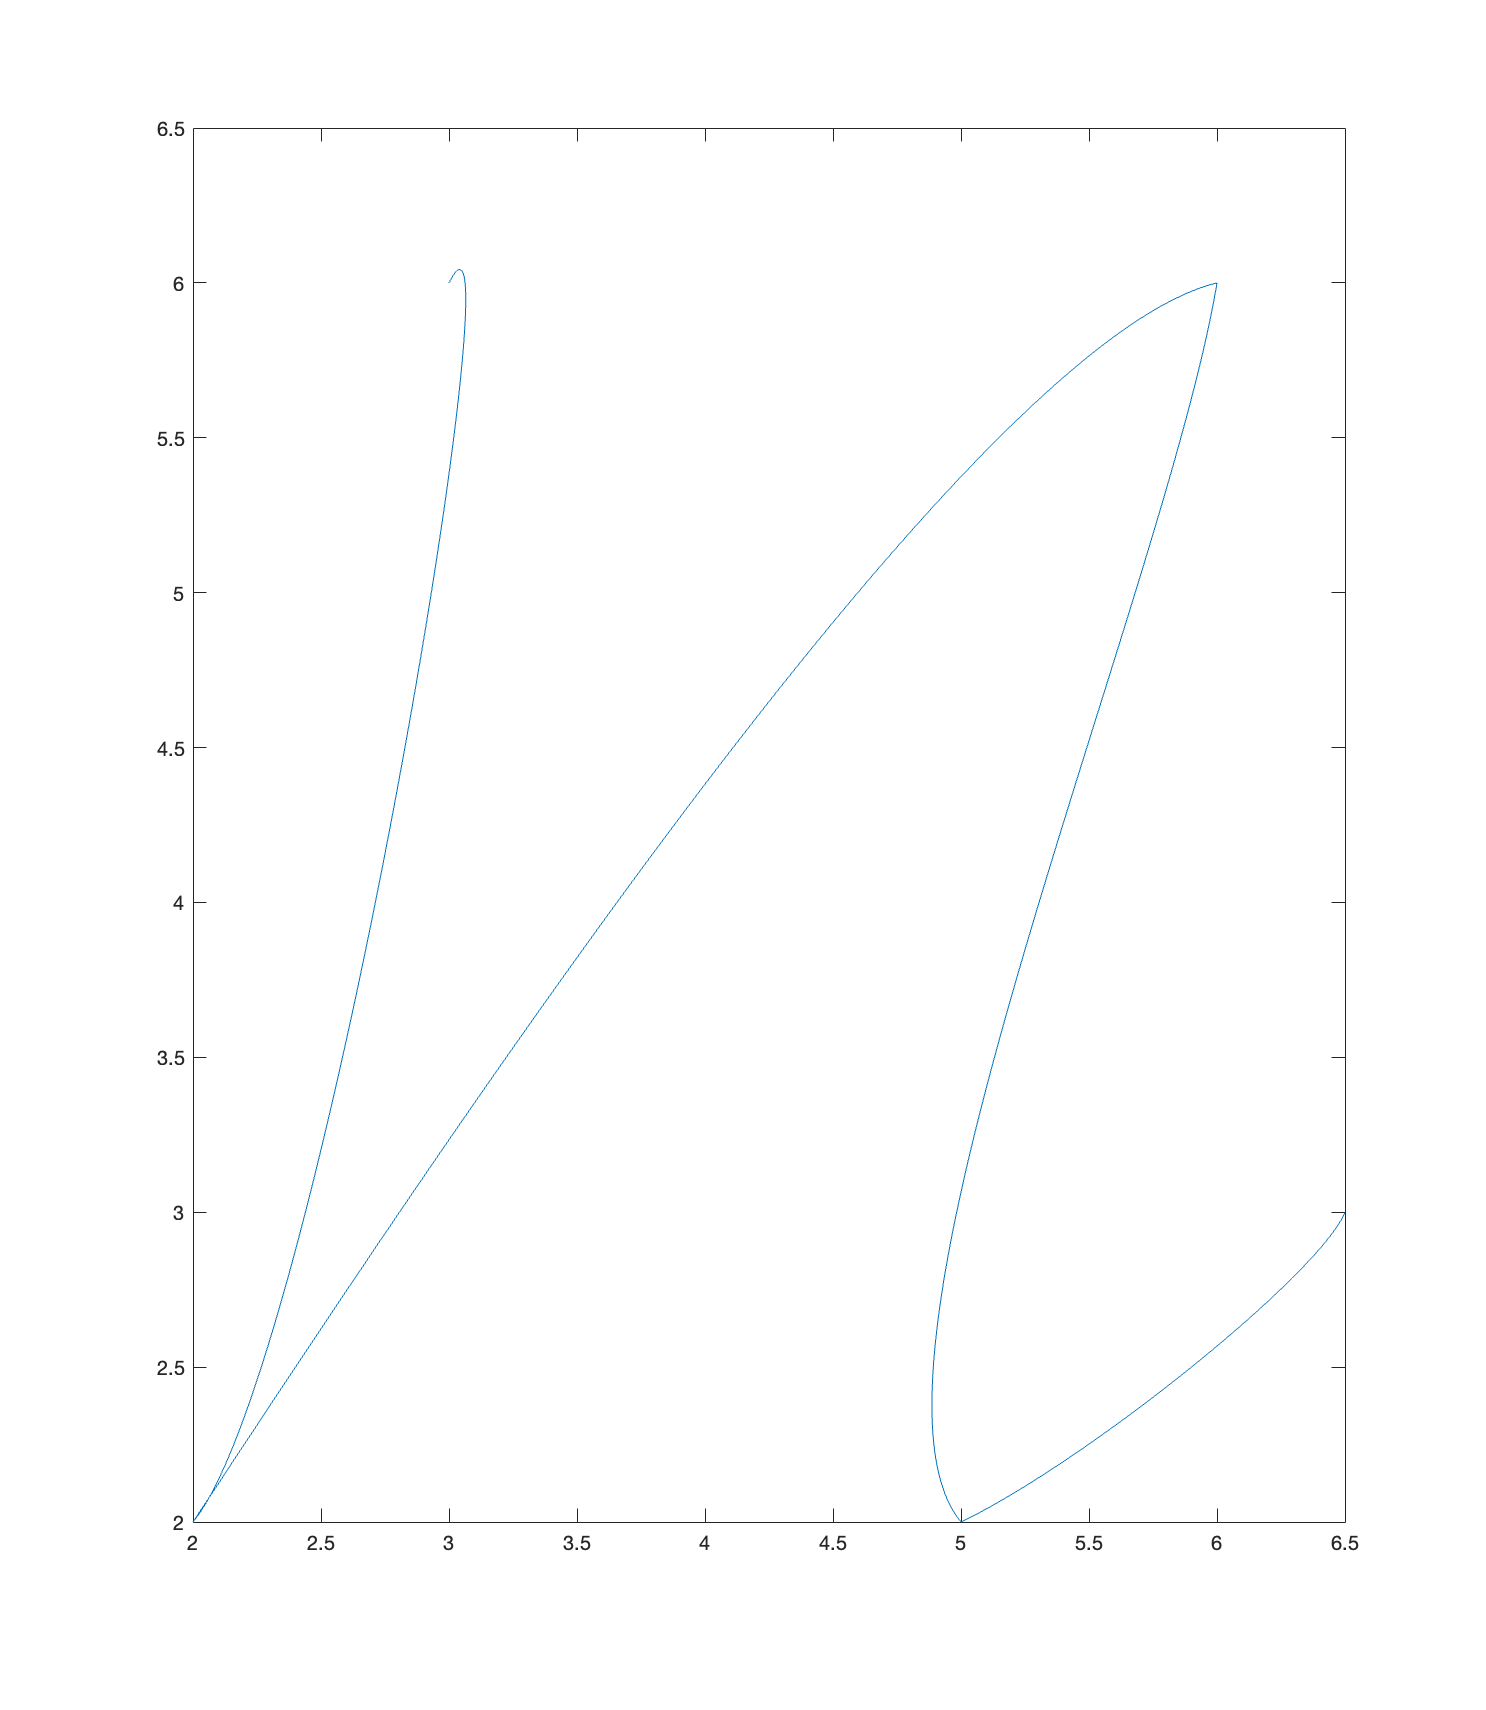
\includegraphics[height=\textwidth]{./figures/letterN.png}

\textbf{Exercise 5}: Suppose a cubic Bezier polynomial is placed through $(u_{0}, v_{0})$ and $(u_{3}, v_{3})$ with guidepoints $(u_{1}, v_{1})$ and $(u_{2}, v_{2})$, respectively.
    \begin{itemize}
        \item [(a)] Derive the parametric equations for $u(t)$ and $v(t)$ assuming that 
            \begin{equation*}
                u(0) = u_{0}, \, u(1) = u_{3}, \, u^{\prime}(0) = u_{1} - u_{0}, \, u^{\prime}(1) = u_{3} - u_{2}
            \end{equation*}
        and
            \begin{equation*}
                v(0) = v_{0}, \, v(1) = v_{3}, \, v^{\prime}(0) = v_{1} - v_{0}, \, v^{\prime}(1) = v_{3} - v_{2}
            \end{equation*}
        \begin{answer}
            We can use the formula for the parametric Bezier polynomial:
                \begin{align*}
                    u(t) &= [2(u_{0} - u_{3}) + 3(u^{\prime}(0) - u^{\prime}(1))]t^{3} + [3(u_{3} - u_{0}) - 3(-u^{\prime}(1) + 2u^{\prime}(0))]t^{2} + u^{\prime}(0)t + u_{0} \\
                    v(t) &= [2(v_{0} - v_{3}) + 3(v^{\prime}(0) - v^{\prime}(1))]t^{3} + [3(v_{3} - v_{0}) - 3(-v^{\prime}(1) + 2v^{\prime}(0))]t^{2} + v^{\prime}(0)t + v_{0}    
                \end{align*}
            Then substitute in the rest, and that is our answer.
        \end{answer}
    \end{itemize}

\newpage
\section*{Exercise Set 4.1}
\hrule

\textbf{Exercise 2}: Use the forward-difference formulas and backward-difference formulas to determine each missing entry in the following tables.
    \begin{itemize}
        \item [(b)] \begin{align*}
            \begin{array}{ c c c }
                x   & f(x)   & f^{\prime}(x) \\
                1.0 & 1.0000 &               \\
                1.2 & 1.2625 &               \\
                1.4 & 1.6595 &                 
            \end{array}
        \end{align*}
        \begin{answer}
            The formula is given by:
                \begin{equation*}
                    f^{\prime}(x) = \dfrac{f(x + h) - f(x)}{h} - \dfrac{h}{2}f^{\prime\prime}(\mathcal{E})
                \end{equation*}
            Then:
                \begin{equation*}
                    f^{\prime}(1.0) \approx \dfrac{f(1.0 + .2) - f(1.0)}{.2} = \dfrac{1.2625 - 1.0000}{.2} = 0.2625 / 0.2 = 1.3125
                \end{equation*}
            and
                \begin{equation*}
                    f^{\prime}(1.2) \approx \dfrac{f(1.2 + .2) - f(1.2)}{.2} = \dfrac{1.6595 - 1.2625}{.2} = 1.985
                \end{equation*}
            For the last one, we need to use the backward difference:
                \begin{equation*}
                    f^{\prime}(1.4) \approx \dfrac{f(1.4 - .2) - f(1.4)}{-.2} = \dfrac{1.2625 - 1.6595}{-.2} = 1.985
                \end{equation*}
            So these are the table entries.
        \end{answer}
    \end{itemize}

\textbf{Exercise 4}: The data in Exercise $2$ were taken from the following functions. Compute the actual errors in Exercise $2$ and find error bounds using the error formulas.
    \begin{itemize}
        \item [(b)] $f(x) = x^{2} \ln{x} + 1$
    \end{itemize}
    \begin{answer}
        I got
            \begin{align*}
                \begin{array}{ c c }
                    x   & f^{\prime}(x) \\
                    1.0 & 1             \\
                    1.2 & 1.63757173631 \\
                    1.4 & 1.98214708762   
                \end{array}
            \end{align*}
        So for the errors:
            \begin{align*}
                \left\lvert \dfrac{1 - 1.3125}{1.3125} \right\rvert           &= 0.23809523809524   \\
                \left\lvert \dfrac{1.985 - 1.63757173631}{1.985} \right\rvert &= 0.1750268330932    \\
                \left\lvert \dfrac{1.985 - 1.98214708762}{1.985} \right\rvert &= 0.0014372354559194   
            \end{align*}
        The error is bounded by
            \begin{equation*}
                \left\lvert \dfrac{f^{\prime\prime}(\mathcal{E})}{2} \right\rvert
            \end{equation*}
        where $\mathcal{E} \in [x_{0}, x_{0} + h]$. The second derivative is given as
            \begin{equation*}
                2\ln{x} + 3
            \end{equation*}
        Since $\ln{x}$ is increasing, we just need to calculate it at the left endpoint for our approximation interval. Here are the error bounds:
            \begin{align*}
                \left\lvert \dfrac{2\ln{1.2} + 3}{2} \right\rvert &= 1.68232155679 \\
                \left\lvert \dfrac{2\ln{1.4} + 3}{2} \right\rvert &= 1.83647223662 \\
                \left\lvert \dfrac{2\ln{1.4} + 3}{2} \right\rvert &= 1.83647223662   
            \end{align*}
    \end{answer}

\textbf{Exercise 6}: Use the most accurate three-point formula to determine each missing entry in the following tables.
    \begin{itemize}
        \item [(d)] \begin{align*}
            \begin{array}{ c c c }
                x    & f(x)     & f^{\prime}(x) \\
                -2.7 & 0.054797 &               \\
                -2.5 & 0.11342  &               \\
                -2.3 & 0.65536  &               \\
                -2.1 & 0.98472  &                 
            \end{array}
        \end{align*}
        \begin{answer}
            We will use the three-point endpoint formula for $-2.7, -2.1$ and the three-point midpoint formula for $-2.5, -2.3$. We have the formulas as:
                \begin{align*}
                    f^{\prime}(x_{0}) &= \dfrac{1}{2h}[-3f(x_{0}) + 4f(x_{0} + h) - f(x_{0} + 2h)] + \dfrac{h^{2}}{3}f^{(3)}(\mathcal{E}_{0}) \\
                    f^{\prime}(x_{0}) &= \dfrac{1}{2h}[f(x_{0} + h) - f(x_{0} - h)] - \dfrac{h^{2}}{6}f^{(3)}(\mathcal{E}_{0})                  
                \end{align*}
            Then for $-2.7$:
                \begin{align*}
                    f^{\prime}(-2.7) &= \dfrac{1}{2 \cdot .2}[-3(0.054797) + 4(0.11342) - 0.65536] \\
                                     &= \dfrac{1}{.4} (-0.164391 + 0.45368 - 0.65536)              \\
                                     &= 2.5 * (-0.164391 + 0.45368 - 0.65536)                      \\
                                     &= -0.9151775                                                   
                \end{align*}
            for $-2.5$:
                \begin{align*}
                    f^{\prime}(-2.5) &= \dfrac{1}{2 \cdot .2}[0.65536 - 0.054797] \\
                                     &= \dfrac{1}{.4}(0.600563)                  \\
                                     &= 2.5 * 0.600563                           \\
                                     &= 0.9151775                                  
                \end{align*}
            for $-2.3$:
                \begin{align*}
                    f^{\prime}(-2.3) &= \dfrac{1}{2 \cdot .2}[0.98472 - 0.11342] \\
                                     &= \dfrac{1}{.4}(0.8713)                    \\
                                     &= 2.5 * 0.8713                             \\
                                     &= 2.17825                                     
                \end{align*}
            and finally for $-2.1$:
                \begin{align*}
                    f^{\prime}(-2.1) &= \dfrac{1}{2 \cdot -.2}[-3(0.98472) + 4(0.65536) - 0.11342] \\
                                     &= \dfrac{-1}{.4}[-2.95416 + 2.62144 - 0.11342]               \\
                                     &= -2.5(-0.44614)                                             \\
                                     &= 1.11535                                                      
                \end{align*}
        \end{answer}
    \end{itemize}

\textbf{Exercise 8}: The data in Exercise $6$ were taken from the following functions. Compute the actual errors in Exercise $6$ and find error bounds using the error formulas.
    \begin{itemize}
        \item [(d)] $f(x) = (\cos{3x})^{2} - e^{2x}$.
            \begin{answer}
                The derivatives that I got are: 
                    \begin{align*}
                        \begin{array}{ c c }
                            x    & f^{\prime}(x)   \\
                            -2.7 & -1.42629912108  \\
                            -2.5 & 1.93738762647   \\
                            -2.3 & 2.81098333684   \\
                            -2.1 & 0.0708779880225   
                        \end{array}
                    \end{align*}
                So calculating the errors:
                    \begin{align*}
                        \left\lvert \dfrac{-0.9151775 + 1.42629912108}{-0.9151775} \right\rvert &= 0.55849452273466 \\
                        \left\lvert \dfrac{0.9151775 - 1.93738762647}{0.9151775} \right\rvert   &= 1.116952860467   \\
                        \left\lvert \dfrac{2.17825 - 2.81098333684}{2.17825} \right\rvert       &= 0.29047783167221 \\
                        \left\lvert \dfrac{1.11535 - 0.0708779880225}{1.11535} \right\rvert     &= 0.94096577655631   
                    \end{align*}
                The error is bounded by
                    \begin{equation*}
                        \dfrac{h^{2}}{3} f^{(3)}(\mathcal{E})
                    \end{equation*}
                for $\mathcal{E}$ in the interval $[x_{0}, x_{0} + 2h]$ or $[x_{0} - h, x_{0} + h]$ depending on the approximation method.
            \end{answer}
    \end{itemize}

\textbf{Exercise 24}: Derive an $\mathcal{O}(h^{4})$ five-point formula to approximate $f^{\prime}(x_{0})$ that uses $f(x_{0} - h), f(x_{0}), f(x_{0} + h), f(x_{0} + 2h)$, and $f(x_{0} + 3h)$.
    \begin{answer}
        
    \end{answer}

\textbf{Exercise 28}: Derive a method for approximating $f^{\prime\prime\prime}(x_{0})$ whose error term is of order $h^{2}$ by expanding the function $f$ in a fourth Taylor polynomial about $x_{0}$ and evaluating at $x_{0} \pm h$ and $x_{0} \pm 2h$.

\newpage
\section*{Exercise Set 4.2}
\hrule

\textbf{Exercise 1}: Apply the extrapolation process described in Example $1$ to determine $N_{3}(h)$, an approximation to $f^{\prime}(x_{0})$, for the following functions and step sizes.
    \begin{itemize}
        \item [(b)] $f(x) = x + e^{x}, x_{0} = 0.0, h = 0.4$
    \end{itemize}
    \begin{answer}
        I got $N_{3}(h) = 2.0554$. Here is my code:
        \inputminted{matlab}{./code/Derivative/ThreePointEndpoint.m}
        \inputminted{matlab}{./code/Derivative/ThreePointMidpoint.m}
        \inputminted{matlab}{./code/Derivative/approxDerive.m}
        \inputminted{matlab}{./code/Extrapolation/Extrapolate.m}
        \inputminted{matlab}{./code/script2.m}
    \end{answer}

\textbf{Exercise 2}: Add another line to the extrapolation table in Exercise $1$ to obtain the approximation $N_{4}(h)$.
    \begin{itemize}
        \item [(b)] $f(x) = x + e^{x}, x_{0} = 0.0, h = 0.4$
    \end{itemize}
    \begin{answer}
        I got $N_{4}(h) = 2.0291$. Here is my code:
        \inputminted{matlab}{./code/Derivative/ThreePointEndpoint.m}
        \inputminted{matlab}{./code/Derivative/ThreePointMidpoint.m}
        \inputminted{matlab}{./code/Derivative/approxDerive.m}
        \inputminted{matlab}{./code/Extrapolation/Extrapolate.m}
        \inputminted{matlab}{./code/script3.m}
    \end{answer}

\textbf{Exercise 5}: The following data give approximations to the integral
    \begin{equation*}
        M = \int_{0}^{\pi} \sin{x} \, \dd{x}
    \end{equation*}
    \begin{equation*}
        N_{1}(h) = 1.570796, \, N_{1}\left(\dfrac{h}{2}\right) = 1.896119, \, N_{1}\left(\dfrac{h}{4}\right) = 1.974232, \, n_{1}\left(\dfrac{h}{8}\right) = 1.993570
    \end{equation*}
Assuming $M = N_{1}(h) + K_{1}h^{2} + K_{2}h^{4} + K_{3}h^{6} + K_{4}h^{8} + \mathcal{O}(h^{10})$, construct an extrapolation table to determine $N_{4}(h)$.
    \begin{answer}
        I got $N_{4}(h) = 2.0000$. Here is my code:
        \inputminted{matlab}{./code/Derivative/ThreePointEndpoint.m}
        \inputminted{matlab}{./code/Derivative/ThreePointMidpoint.m}
        \inputminted{matlab}{./code/Derivative/approxDerive.m}
        \inputminted{matlab}{./code/Extrapolation/Extrapolate.m}
        \inputminted{matlab}{./code/script4.m}
    \end{answer}

\textbf{Exercise 8}: The forward-difference formula can be expressed as 
    \begin{equation*}
        f^{\prime}(x_{0}) = \dfrac{1}{h}[f(x_{0} + h) - f(x_{0})] - \dfrac{h}{2}f^{\prime\prime}(x_{0}) - \dfrac{h^{2}}{6}f^{\prime\prime\prime}(x_{0}) + \mathcal{O}(h^{3})
    \end{equation*}
Use extrapolation to derive an $\mathcal{O}(h^{3})$ formula for $f^{\prime}(x_{0})$.
    \begin{answer}
        Let 
            \begin{equation*}
                N_{1}(h) = \dfrac{1}{h}[f(x_{0} + h) - f(x_{0})]
            \end{equation*}
        as our initial guess. Then we see that it has an error of 
            \begin{equation*}
                -\dfrac{h}{2}f^{\prime\prime}(x_{0}) - \dfrac{h^{2}}{6}f^{\prime\prime\prime}(x_{0}) + \mathcal{O}(h^{3})
            \end{equation*}
        To get rid of the $\frac{h}{2}$ error, we use
            \begin{equation*}
                N_{2}(h) = N_{1}\left(\dfrac{h}{2}\right) + \left[N_{1}\left(\dfrac{h}{2}\right) - N_{1}(h)\right]
            \end{equation*}
        So
            \begin{align*}
                N_{2}(h) &= \dfrac{2}{h}\left[f\left(x_{0} + \dfrac{h}{2}\right) - f(x_{0})\right] + \left[\dfrac{2}{h}\left[f\left(x_{0} + \dfrac{h}{2}\right) - f(x_{0})\right] - \dfrac{1}{h}[f(x_{0} + h) - f(x_{0})]\right]   
            \end{align*}
        And so on. We do the same process but then with:
            \begin{equation*}
                N_{3}(h) = N_{2}\left(\dfrac{h}{2}\right) + \dfrac{1}{15}\left[N_{2}\left(\dfrac{h}{2}\right) - N_{2}(h)\right]
            \end{equation*}
        to get our $\mathcal{O}(h^{3})$ approximation.
    \end{answer}

\textbf{Exercise 9}: Suppose that $N(h)$ is an approximation to $M$ for every $h > 0$ and that
    \begin{equation*}
        M = N(h) + K_{1}h + K_{2}h^{2} + K_{3}h^{3} + \cdots,
    \end{equation*}
for some constant $K_{1}, K_{2}, K_{3}, \ldots$. Use the values $N(h), N(\frac{h}{3}),$ and $N(\frac{h}{9})$ to produce an $\mathcal{O}(h^{3})$ approximation to $M$.
    \begin{answer}
        We have that
            \begin{equation*}
                M = N_{1}\left(\dfrac{h}{3}\right) + K_{1}\left(\dfrac{h}{3}\right) + K_{2} \left(\dfrac{h}{3}\right)^{2} + \cdots
            \end{equation*}
        Then
            \begin{equation*}
                3M = 3N_{1}\left(\dfrac{h}{3}\right) + 3K_{1}\left(\dfrac{h}{3}\right) + 3K_{2}\left(\dfrac{h}{3}\right)^{2} + \cdots
            \end{equation*}
        so
            \begin{equation*}
                2M = 3N_{1}\left(\dfrac{h}{3}\right) - N_{1}(h) + K_{2}\left(\dfrac{h^{2}}{3}\right) - K_{2}h^{2} + \cdots
            \end{equation*}
        and
            \begin{equation*}
                M = \dfrac{1}{2}\left(3N_{1}\left(\dfrac{h}{3}\right) - N_{1}(h)\right) - \dfrac{1}{3}K_{2}h^{2} + \cdots
            \end{equation*}
        Now let
            \begin{equation*}
                N_{2}(h) = \dfrac{1}{2}\left(3N_{1}\left(\dfrac{h}{3}\right) - N_{1}(h)\right)
            \end{equation*}
        We have:
            \begin{equation*}
                N_{2}\left(\dfrac{h}{3}\right) = \dfrac{1}{2}\left(3N_{1}\left(\dfrac{h}{9}\right) - N_{1}\left(\dfrac{h}{3}\right)\right)
            \end{equation*}
        Notice that now we have:
            \begin{align*}
                M &= N_{2}(h) - \dfrac{1}{3}K_{2}h^{2}                                 \\
                M &= N_{2}\left(\dfrac{h}{3}\right) - \dfrac{1}{27}K_{2}h^{2} + \cdots   
            \end{align*}
        Then
            \begin{equation*}
                9M = 9N_{2}\left(\dfrac{h}{3}\right) - \dfrac{1}{3}K_{2}h^{2} + \cdots
            \end{equation*}
        and
            \begin{equation*}
                8M = 9N_{3}\left(\dfrac{h}{2}\right) - N_{2}(h)
            \end{equation*}
        So the final $\mathcal{O}(h^{3})$ approximation is
            \begin{equation*}
                \dfrac{9}{8}\left(N_{2}\left(\dfrac{h}{3}\right) - N_{2}(h)\right)
            \end{equation*}
        We can write this in terms of $N_{1}(h), N_{1}(h / 3), N_{1}(h / 9)$:
            \begin{equation*}
                \dfrac{9}{8}\left(\dfrac{1}{2}\left(3N_{1}\left(\dfrac{h}{9}\right) - N_{1}\left(\dfrac{h}{3}\right)\right) - \dfrac{1}{2}\left(3N_{1}\left(\dfrac{h}{3}\right) - N_{1}(h)\right)\right)
            \end{equation*}
    \end{answer}

\textbf{Exercise 14}: Suppose that $N_{1}(h)$ is a formula that produces $\mathcal{O}(h)$ approximations to a number $M$ and that 
    \begin{equation*}
        M = N_{1}(h) + K_{1}(h) + K_{2}h^{2} + \cdots,
    \end{equation*}
for a collection of positive constants $K_{1}, K_{2}, \ldots$. Then $N_{1}(h), N_{1}(h / 2), N_{1}(h / 4), \ldots$ are all lower bounds for $M$. What can be said about the extrapolated approximations $N_{2}(h), N_{3}(h), \ldots$?

\end{document}
